% !TeX root = ../main.tex

\chapter{文件系统架构设计}
\label{cha:design}

% 本课题采用的设计方案

本课题设计并实现的文件系统大致包含两层:文件系统层和纠删码层。

由于本课题的核心目标是证明利用纠删码提供可用性保障的可行性和评估其相对效率,因此文件系统层直接复用了已有的工作 LocoFS\cite{li2017}。LocoFS 是一个针对元数据操作进行优化的分布式文件系统原型,它的各种逻辑相对简单,方便移植。但是,LocoFS 针对传统低速块设备存储和低速网络设计,对 CPU 资源的使用较为随意;因此本课题在移植 LocoFS 时,重写了其网络通信逻辑,同时优化了读写路径,尽可能降低了网络带宽占用和 CPU 开销。

文件系统的节点分为三类:目录元数据服务器(DMS)、文件元数据服务器(FMS)和文件数据服务器(DS)。其中,DMS 只有一个,负责存放目录元数据和进行目录操作;FMS 可以有多个,负责存放文件元数据和进行文件元数据操作;DS 也可以有多个,负责存储文件数据。在实现时,任何一个 DS 都可以同时充当客户端,与元数据服务器通信,进行各种文件系统操作。

纠删码层对文件系统层提供 4KB 页粒度的数据访问接口。它对用户屏蔽底层 NVM 设备,向用户层提供一个连续的虚拟 NVM 空间。当用户读写某一个虚拟页时,纠删码层自动计算其对应的数据块位置;如果是读操作,则通过 RDMA 读操作取得对应的数据块,解码出原数据块后返回给用户;如果是写操作,则先对数据块进行编码,然后将数据块和纠删码块通过 RDMA 写操作写入到对应的位置上。

整个系统的架构如下图所示:

\begin{figure}[H]
    \centering
    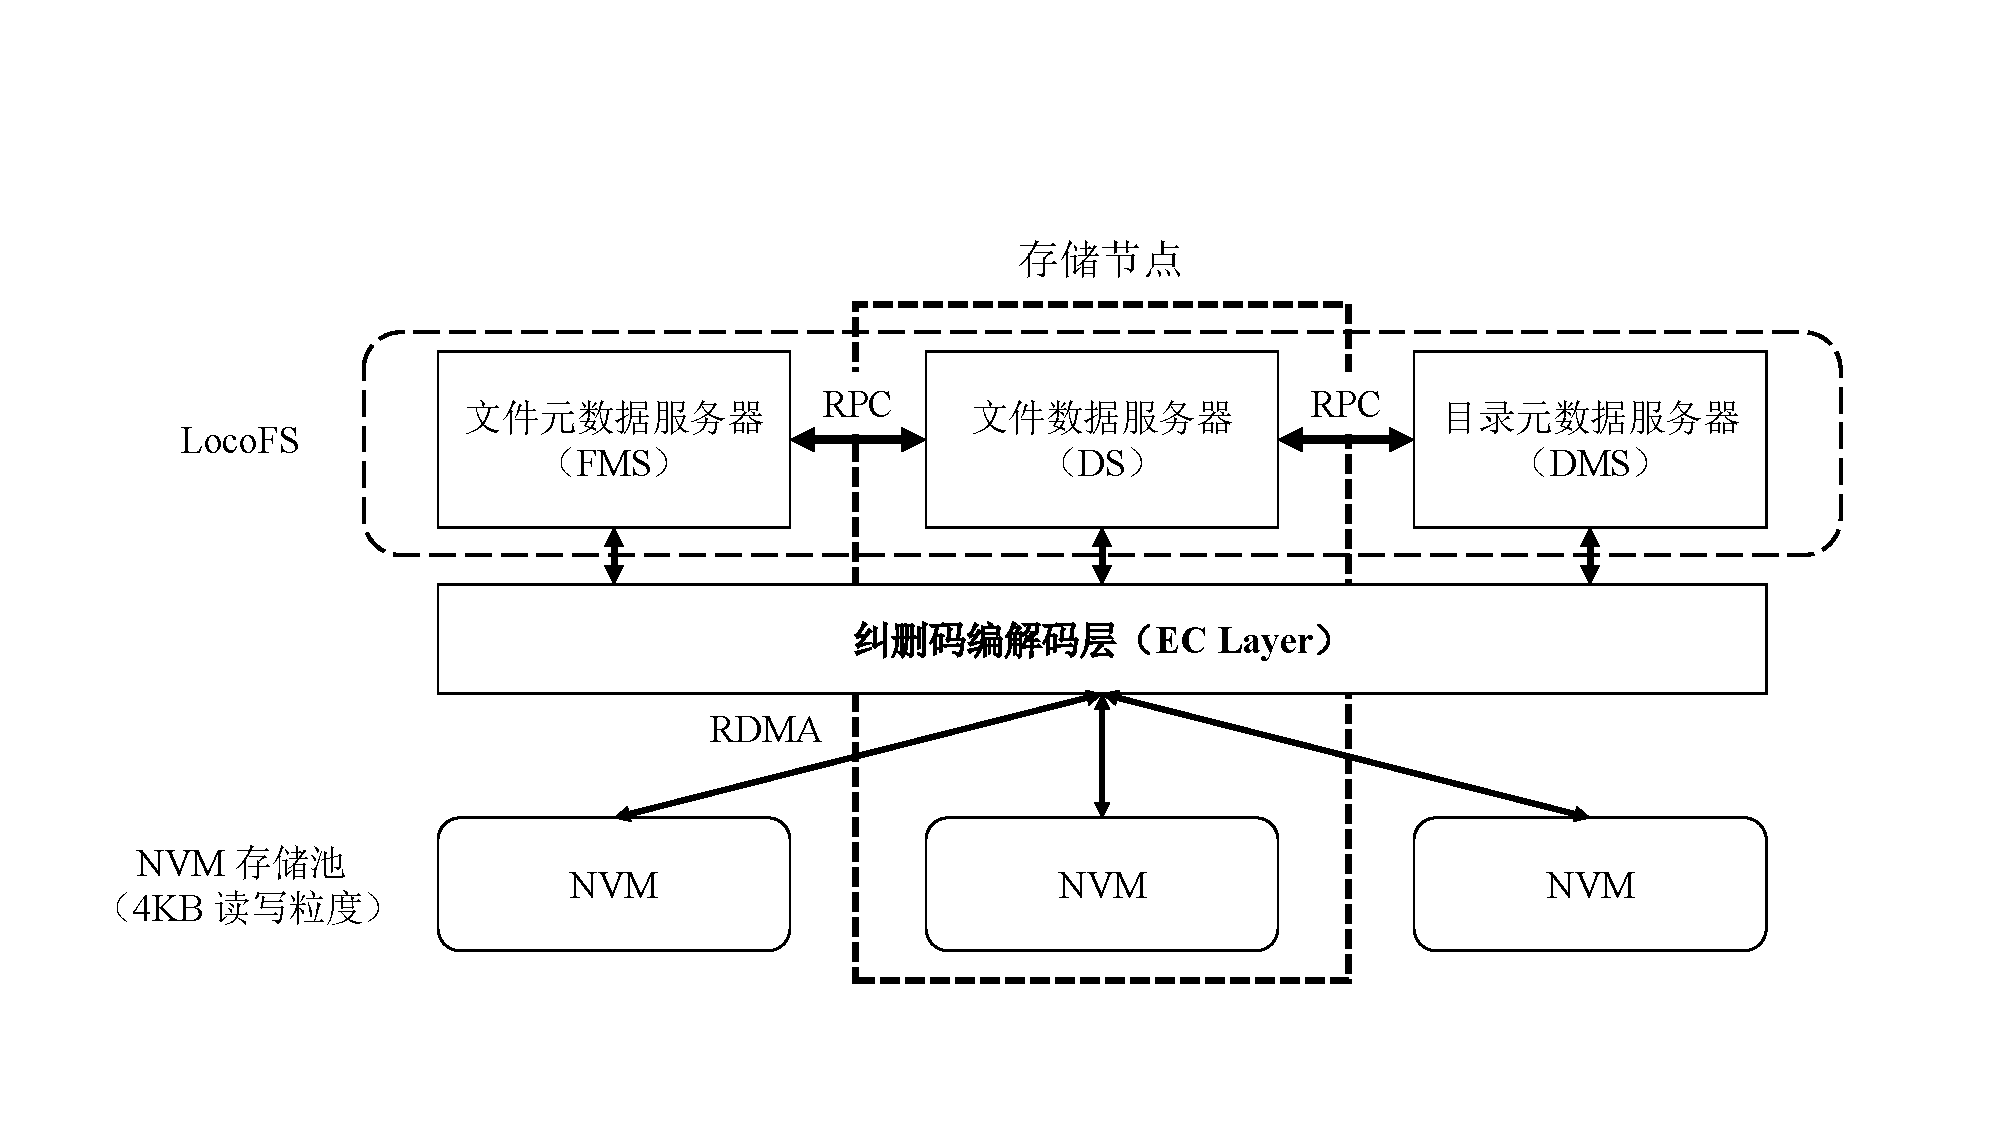
\includegraphics[width=10cm]{galois-structure.pdf}
    \caption{系统架构示意图}
    \label{fig:struct}
\end{figure}

以下各小节将详细说明文件系统的细节设计和优化方案。

\section{纠删码策略的选用}

根据被编码数据块的大小不同,纠删码策略又可细分为两种:

\begin{enumerate}[(1)]
    
    \item \textbf{分组}:被编码的数据块单元大小等于 4KB。以 $RS(4, 2)$ 为例,分组策略对 4 个 4KB 原始数据块进行编码,产生 2 个 4KB 的校验数据块,然后将它们分别存放于 6 个物理上分离的存储设备上。分组的优势是读写时网络访问次数少;劣势是写入操作较为复杂,同时需要额外处理系统降级时的读操作。

    \item \textbf{切块}:被编码的数据块单元大小等于 $\frac{4}{k}$ KB,其中 $k$ 是纠删码的参数。以 $RS(4, 2)$ 为例($k = 4$),切块策略把一个 4KB 原始数据块切分为 4 个 1KB 数据块,对其编码,产生 2 个 1KB 的校验数据块,然后将 6 个 1KB 数据块分别存放于 6 个物理上分离的存储设备上。切块的优势是读写逻辑简单,系统降级情况下读操作不受影响;劣势是读写时需要的网络访问次数较多。

\end{enumerate}

以上两种策略的读写特性如下表所示:


